\chapter{Quality of the data description}
%Plots Ripani/Fedotov integral and differential. Very low $Q^{2}$. $Q^{2}$ dependence.
\label{quality}
As described in Sect.~\ref{unfold}, one can simply unfold the values of the integrated and single-differential cross sections from the EG distributions.  This section presents the plots that illustrate how well the EG describes the input data in the regions, where they exist. All TWOPEG distributions, which are shown below, have been generated in the $F_{flux}=0$ mode.  

Figures~\ref{fig:eg_rip} and \ref{fig:eg_fed} show the comparison between the event distributions of TWOPEG (curves) with the integrated cross sections from the JM model~\cite{Mokeev:2015lda},~\cite{Mokeev:2008iw},~\cite{Mokeev:2012vsa}  (circles) and measured data~\cite{Ripani:2002ss},~\cite{Fedotov:2008aa} (squares) for different values of $Q^2$ for the electroproduction data-sets 1a and 1b, respectively. In Figs.~\ref{fig:eg_rip_095_15875} and \ref{fig:eg_fed_0425_14625} the analogous comparison is made for the single-differential cross sections of these data-sets.

The comparison that is shown in Figs.~\ref{fig:eg_rip_065_17125} and \ref{fig:eg_gol_17125}, corresponds to the $Q^2$ boundaries of the region II in Fig.~\ref{fig:gen_cover}. As it is described in Sect.~\ref{sect:cr_sect_extr_intr}, the five-dimensional cross section in this region is a mixture of the two cross section samples, each scaled from the corresponding $Q^2$ edge at $Q^2 = 0$~GeV$^2$ and $Q^2 = 0.65$~GeV$^2$. The mixing is made in the way that at the $Q^2$ edge the resultant cross section coincides with the corresponding model cross section at this edge (see Eq.~\eqref{eq:q2_dep_fit_sig_t}). Figure~\ref{fig:eg_rip_065_17125} shows the comparison between event distributions of TWOPEG and the single-differential model cross sections at the $Q^2 = 0.65$~GeV$^2$ edge, while Fig.~\ref{fig:eg_gol_17125} shows the same for the $Q^2 = 0$~GeV$^2$ edge. 

The comparison that is shown in Figs.~\ref{fig:eg_rip_130_20625} and \ref{fig:eg_gol_20625}, corresponds to the $Q^2$ boundaries of the region IV in Fig.~\ref{fig:gen_cover}. The same idea of cross section mixing is applied here. Figure~\ref{fig:eg_rip_130_20625} shows the comparison between TWOPEG event distributions and the single-differential experimental cross sections at the $Q^2 = 1.3$~GeV$^2$ edge, while Fig.~\ref{fig:eg_gol_20625} shows the same for the $Q^2 = 0$~GeV$^2$ edge. 

Figure~\ref{fig:eg_ph_point} (upper plot) demonstrates that TWOPEG nicely reproduces the behavior of the total integrated cross section close to $Q^2 = 0$~GeV$^2$. Furthermore, the lower plot in Fig.~\ref{fig:eg_ph_point} shows a typical example of the $Q^2$ dependence of the total cross section. 

In any desired point of the regions 1a, 1b, and 2a in Fig.~\ref{fig:gen_cover} TWOPEG produces the established values of the model cross section. In the regions I, II, and IV the EG gives some cross section estimation based on the cross section in the neighboring areas and can therefore be used as a prediction of a naive model. In other regions the cross section estimates are less reliable, but good enough for the modeling of experiments (efficiency evaluation, background estimation, etc.).  

 %\clearpage
%\newpage

\begin{figure}[!ht]
\begin{center}
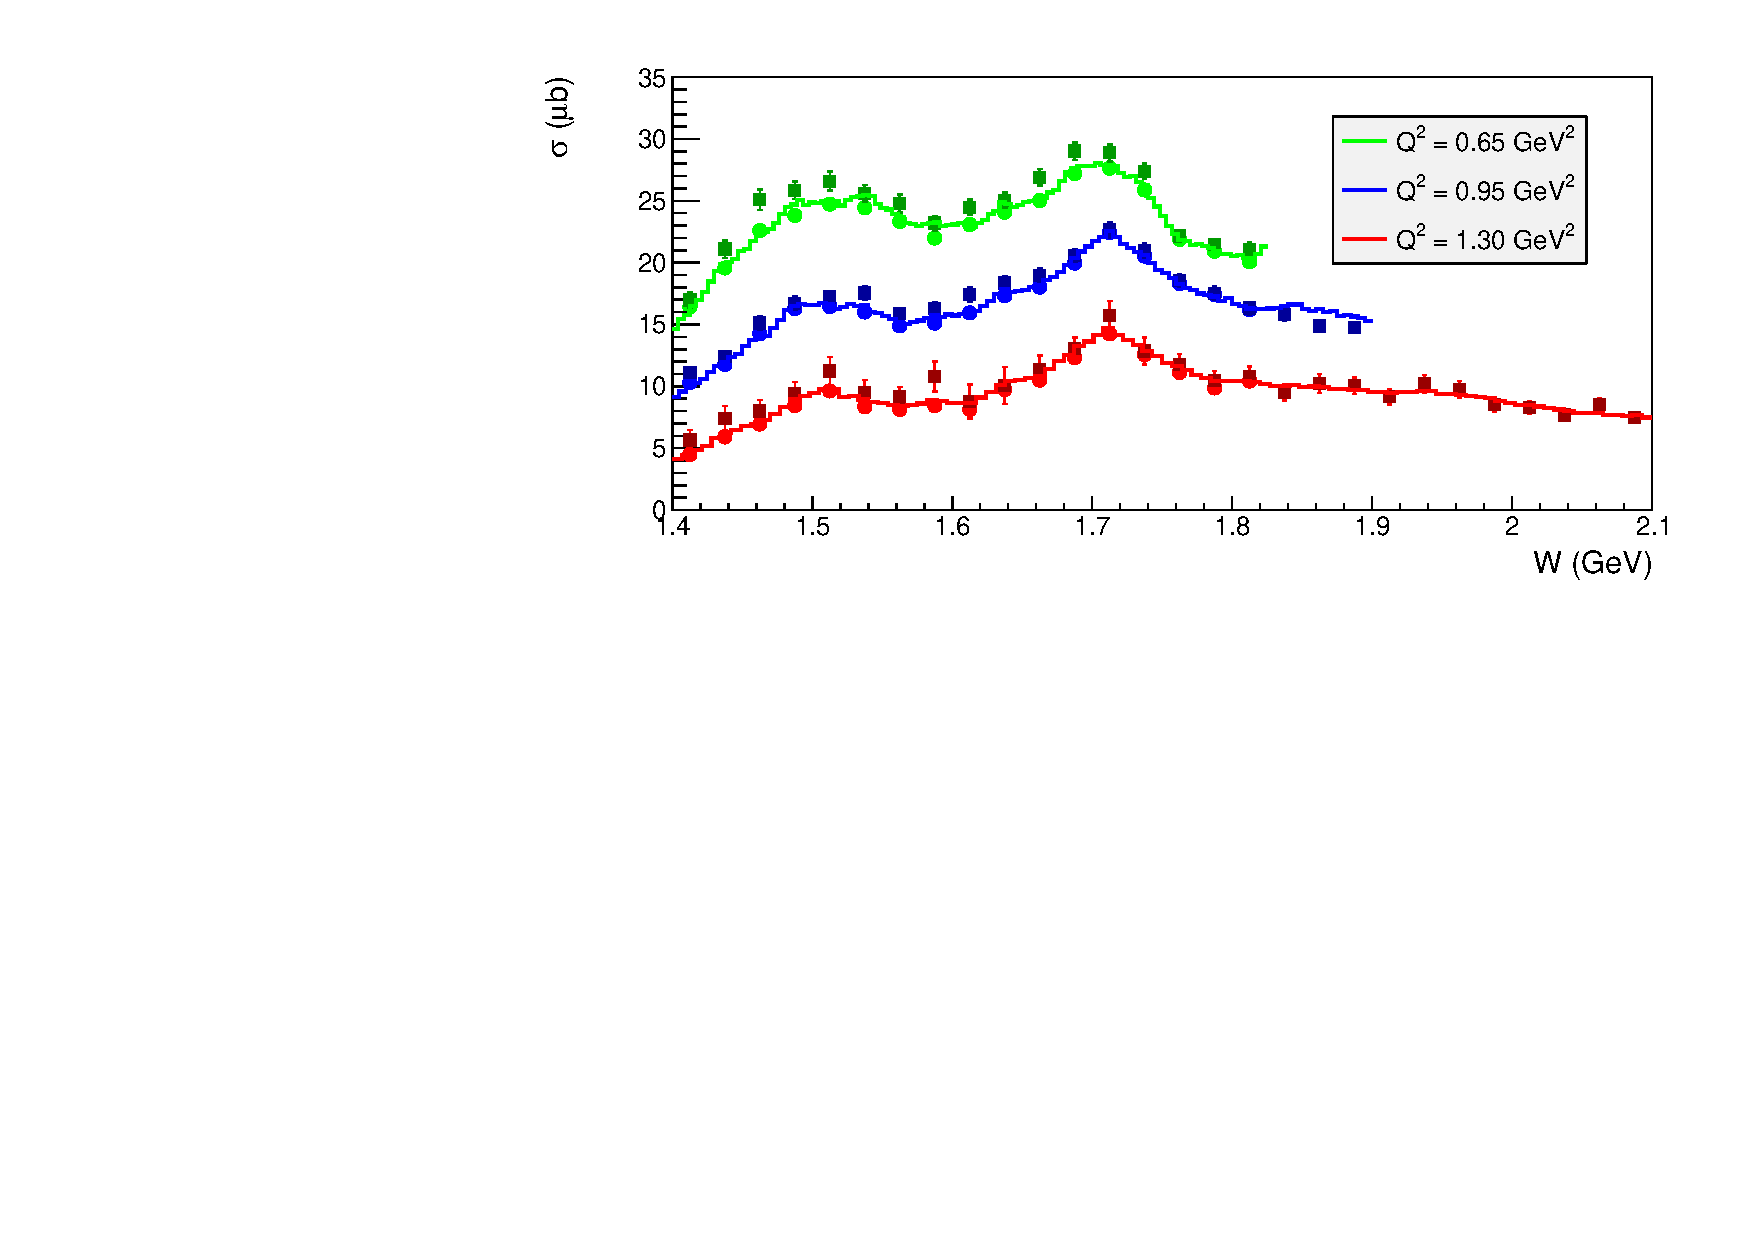
\includegraphics[width=0.75\textwidth]{pictures/quality/ripani_065_095_130_gen_comp.pdf}
\end{center}
\vspace{-0.6cm}
\caption{\small Comparison between event distributions of TWOPEG (curves) for different $Q^2$ bins, the integrated cross sections from the JM model~\cite{Mokeev:2015lda} (circles), and data~\cite{Ripani:2002ss} (squares) for the corresponding three $Q^2$ points at 0.65, 0.95, and 1.3~GeV$^2$. To obtain the green and blue curves the beam energy was set to 2.445 GeV, while for the red one the beam energy was set to 4 GeV. This comparison corresponds to the data-set 1a, which is marked in Fig.~\ref{fig:gen_cover} as the region within the red boundaries. }
\label{fig:eg_rip}
\end{figure}


\begin{figure}[!ht]
\begin{center}
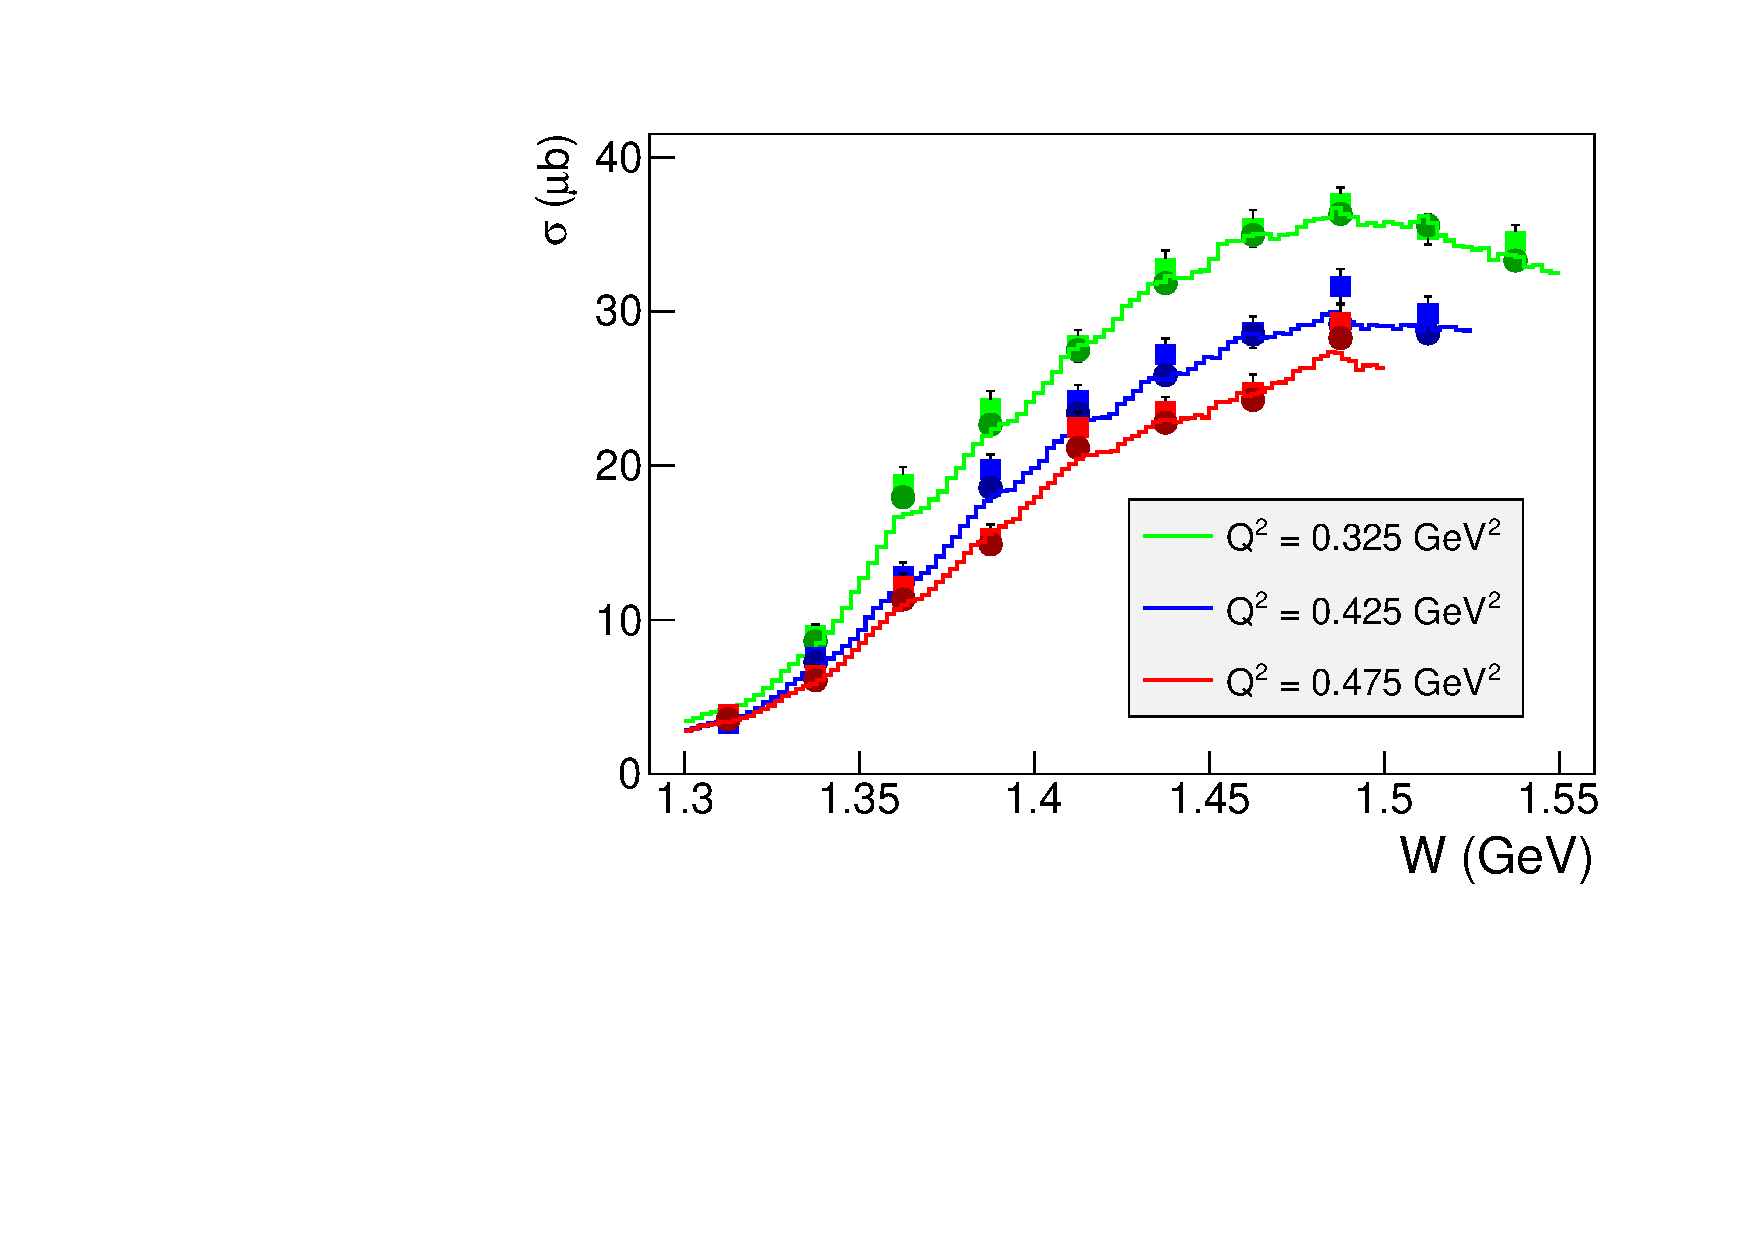
\includegraphics[width=0.6\textwidth]{pictures/quality/fedotov_wdep_3q2bins_gen_comp.pdf}
\end{center}
\vspace{-0.6cm}
\caption{\small Comparison of the TWOPEG event distributions (curves) for different $Q^2$ bins with the integrated cross sections from the JM model~\cite{Mokeev:2008iw},~\cite{Mokeev:2012vsa} (circles) and data~\cite{Fedotov:2008aa} (squares) for the corresponding three $Q^2$ points at 0.325, 0.425, and 0.475~GeV$^2$. The TWOPEG distributions were obtained for $E_{beam} = 1.515$ GeV. This comparison corresponds to the data-set 1b, which is marked in Fig.~\ref{fig:gen_cover} as the region within the lilac boundaries.}
\label{fig:eg_fed}
\end{figure}

\clearpage
\newpage


\begin{figure}[!ht]
\begin{center}
\frame{
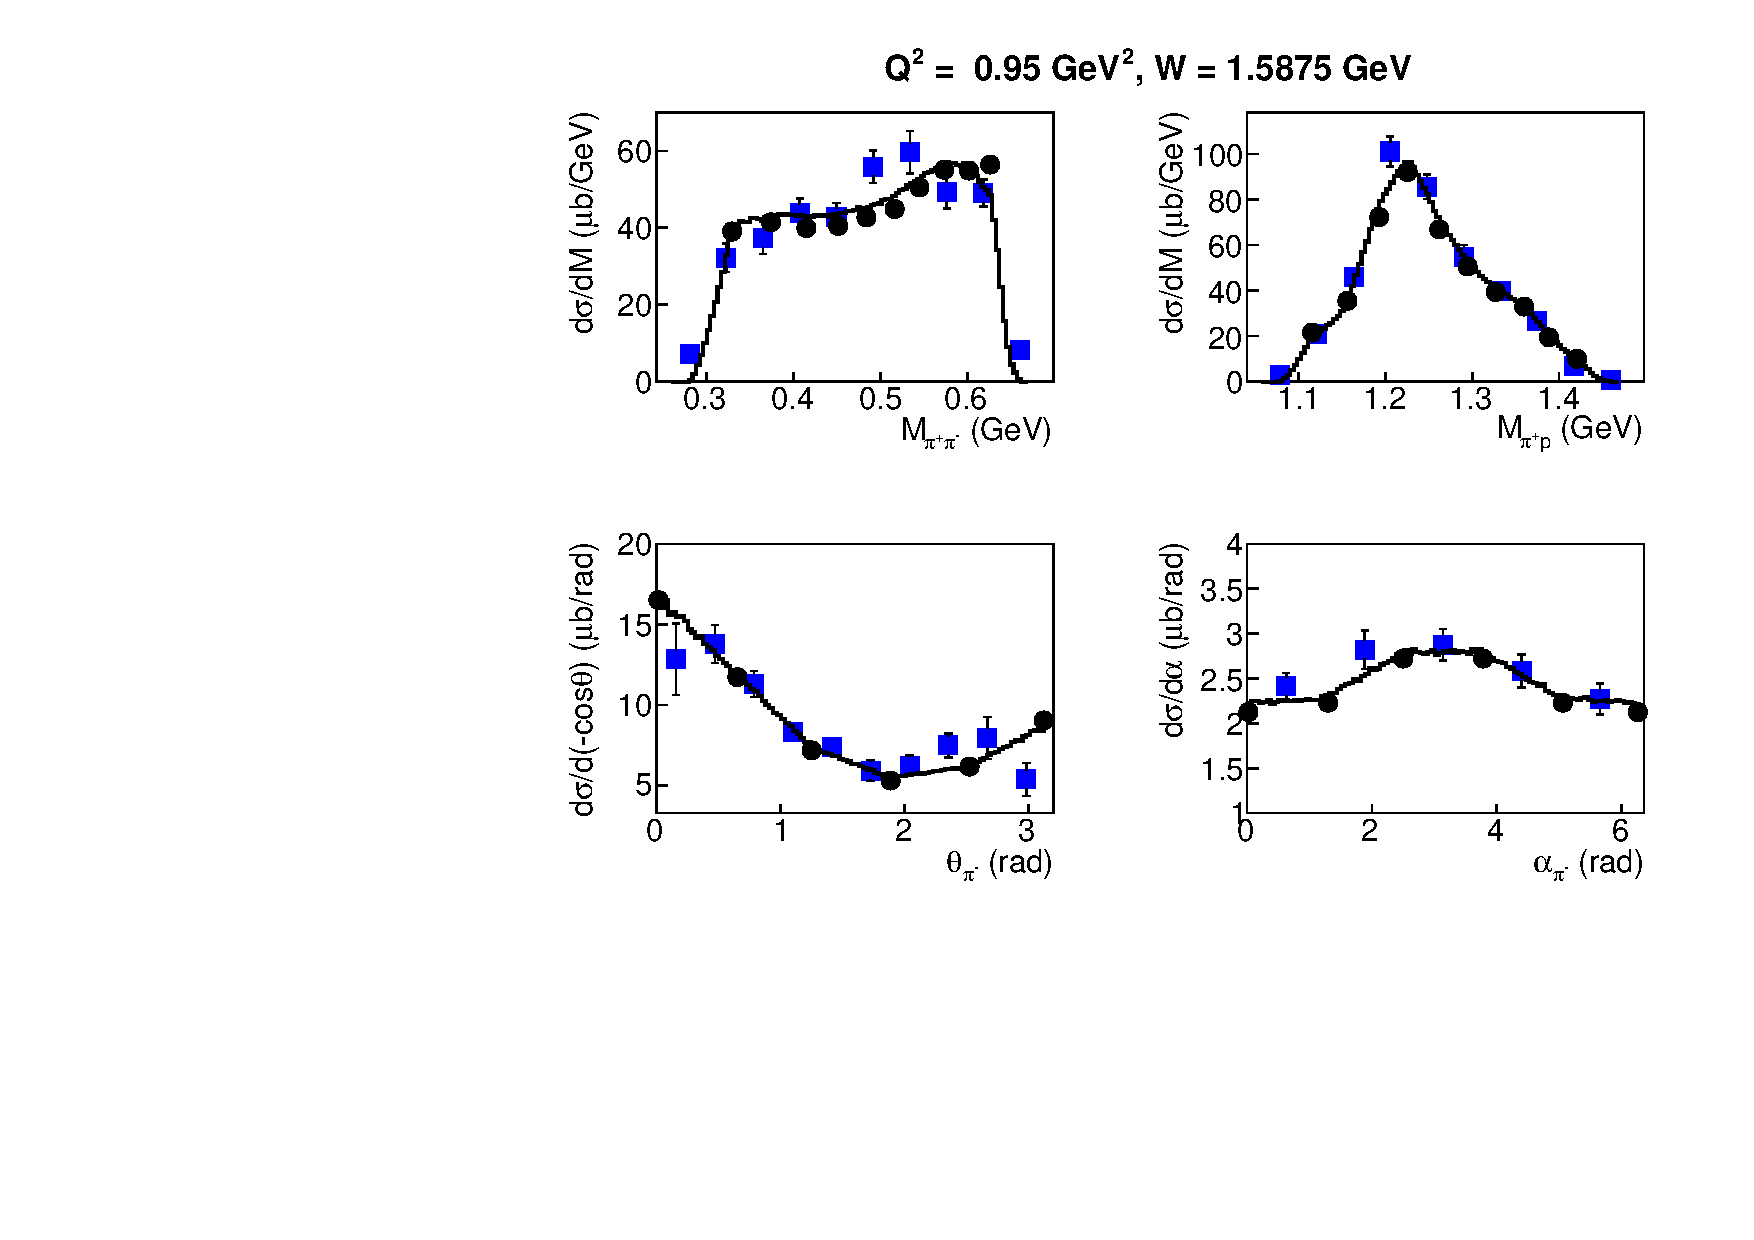
\includegraphics[height=0.45\textwidth]{pictures/quality/rip_095_15875.pdf}
}
\end{center}
\vspace{-0.6cm}
\caption{\small Comparison of the TWOPEG event distributions (curves) for the $W$ bin [1.575,~1.6]~GeV and $Q^2$ bin [0.8,~1.1]~GeV$^2$ with the single-fold differential cross sections from the JM model~\cite{Mokeev:2015lda} (circles) and data~\cite{Ripani:2002ss} (squares) for the $W = 1.5875$~GeV, $Q^2 = 0.95$~GeV$^2$ point. The TWOPEG distributions were obtained for $E_{beam} = 2.445$ GeV. This comparison corresponds to the data-set 1a, which is marked in Fig.~\ref{fig:gen_cover} as the region within the red boundaries.}
\label{fig:eg_rip_095_15875}
\end{figure}



\begin{figure}[!ht]
\begin{center}
\frame{
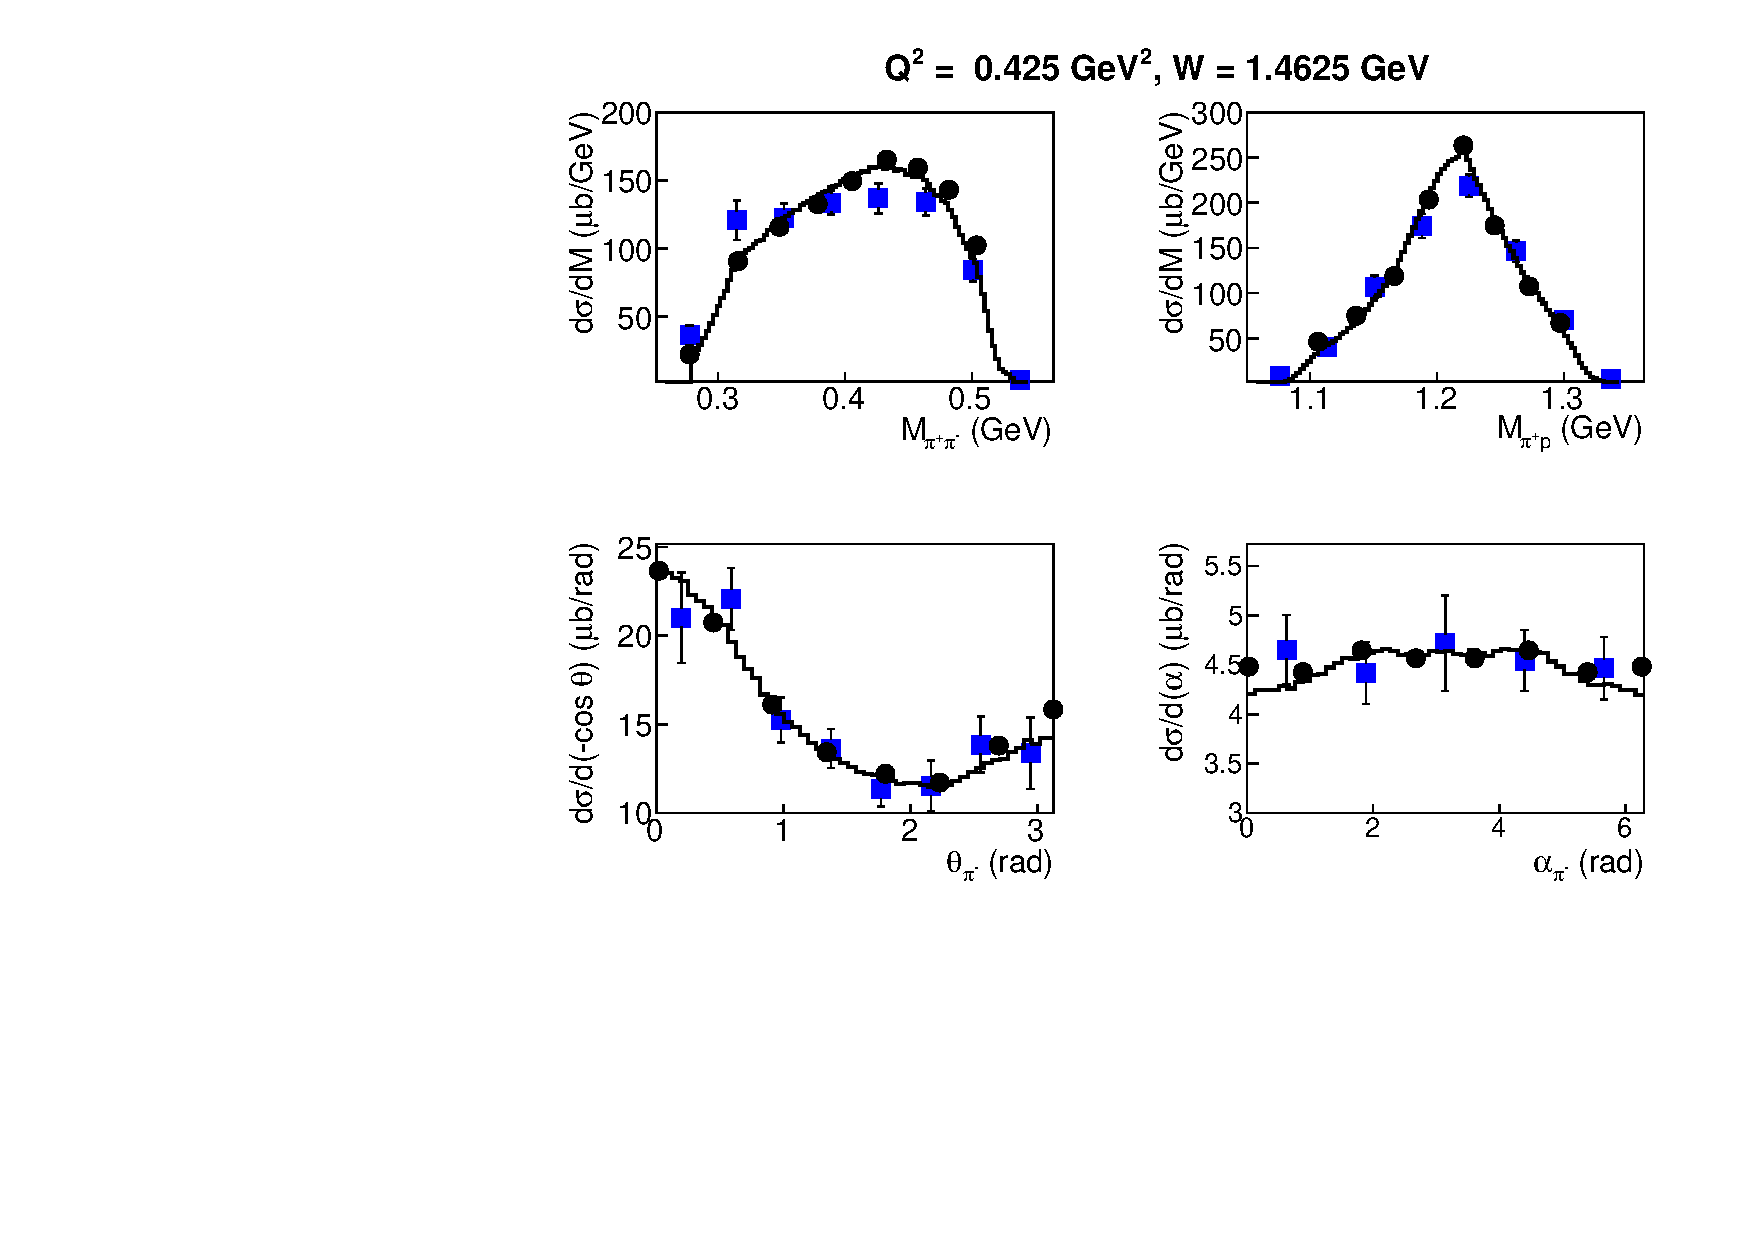
\includegraphics[height=0.45\textwidth]{pictures/quality/fed_0425_14625.pdf}
}
\end{center}
\vspace{-0.6cm}
\caption{\small Comparison of the TWOPEG event distributions (curves) for the $W$ bin [1.45,~1.475]~GeV and $Q^2$ bin [0.4,~0.45]~GeV$^2$ with the single-fold differential cross sections from the JM model~\cite{Mokeev:2008iw},~\cite{Mokeev:2012vsa} (circles) and data~\cite{Fedotov:2008aa} (squares) for the $W = 1.4625$~GeV, $Q^2 = 0.425$~GeV$^2$ point. The TWOPEG distributions were obtained for $E_{beam} = 1.515$ GeV. This comparison corresponds to the data-set 1b, which is marked in Fig.~\ref{fig:gen_cover} as the region within the lilac boundaries.}
\label{fig:eg_fed_0425_14625}
\end{figure}



\begin{figure}[!ht]
\begin{center}
\frame{
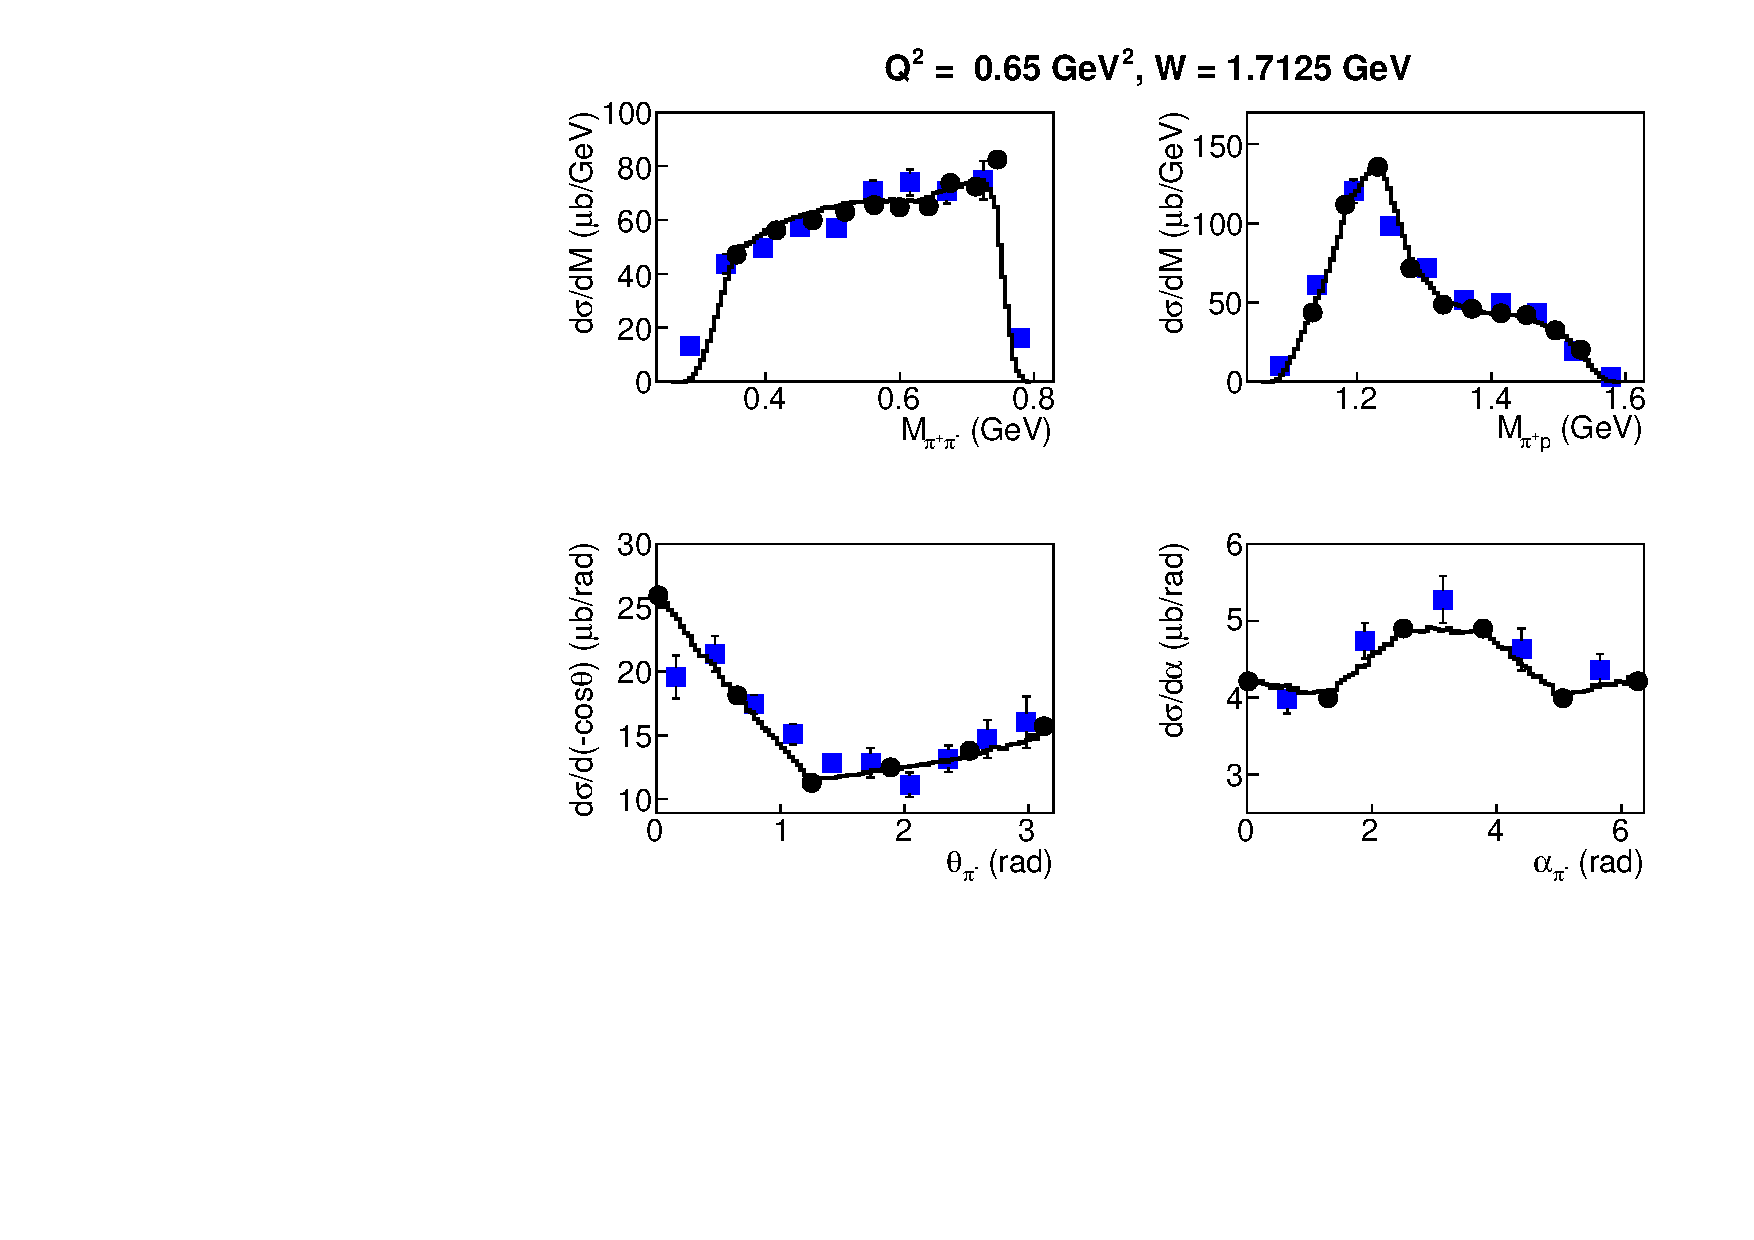
\includegraphics[height=0.45\textwidth]{pictures/quality/rip_065_17125.pdf}
}
\end{center}
\vspace{-0.6cm}
\caption{\small Comparison of the TWOPEG event distributions (curves) for the $W$ bin [1.7,~1.725]~GeV and $Q^2$ bin [0.5,~0.8]~GeV$^2$ with the single-fold differential cross sections from the JM model~\cite{Mokeev:2015lda} (circles) and data~\cite{Ripani:2002ss} (squares) for the $W = 1.7125$~GeV, $Q^2 = 0.65$~GeV$^2$ point. The TWOPEG distributions were obtained for $E_{beam} = 2.445$ GeV. This comparison corresponds to the data-set 1a, which is marked in Fig.~\ref{fig:gen_cover} as the region within the red boundaries.}
\label{fig:eg_rip_065_17125}
\end{figure}



\begin{figure}[!ht]
\begin{center}
\frame{
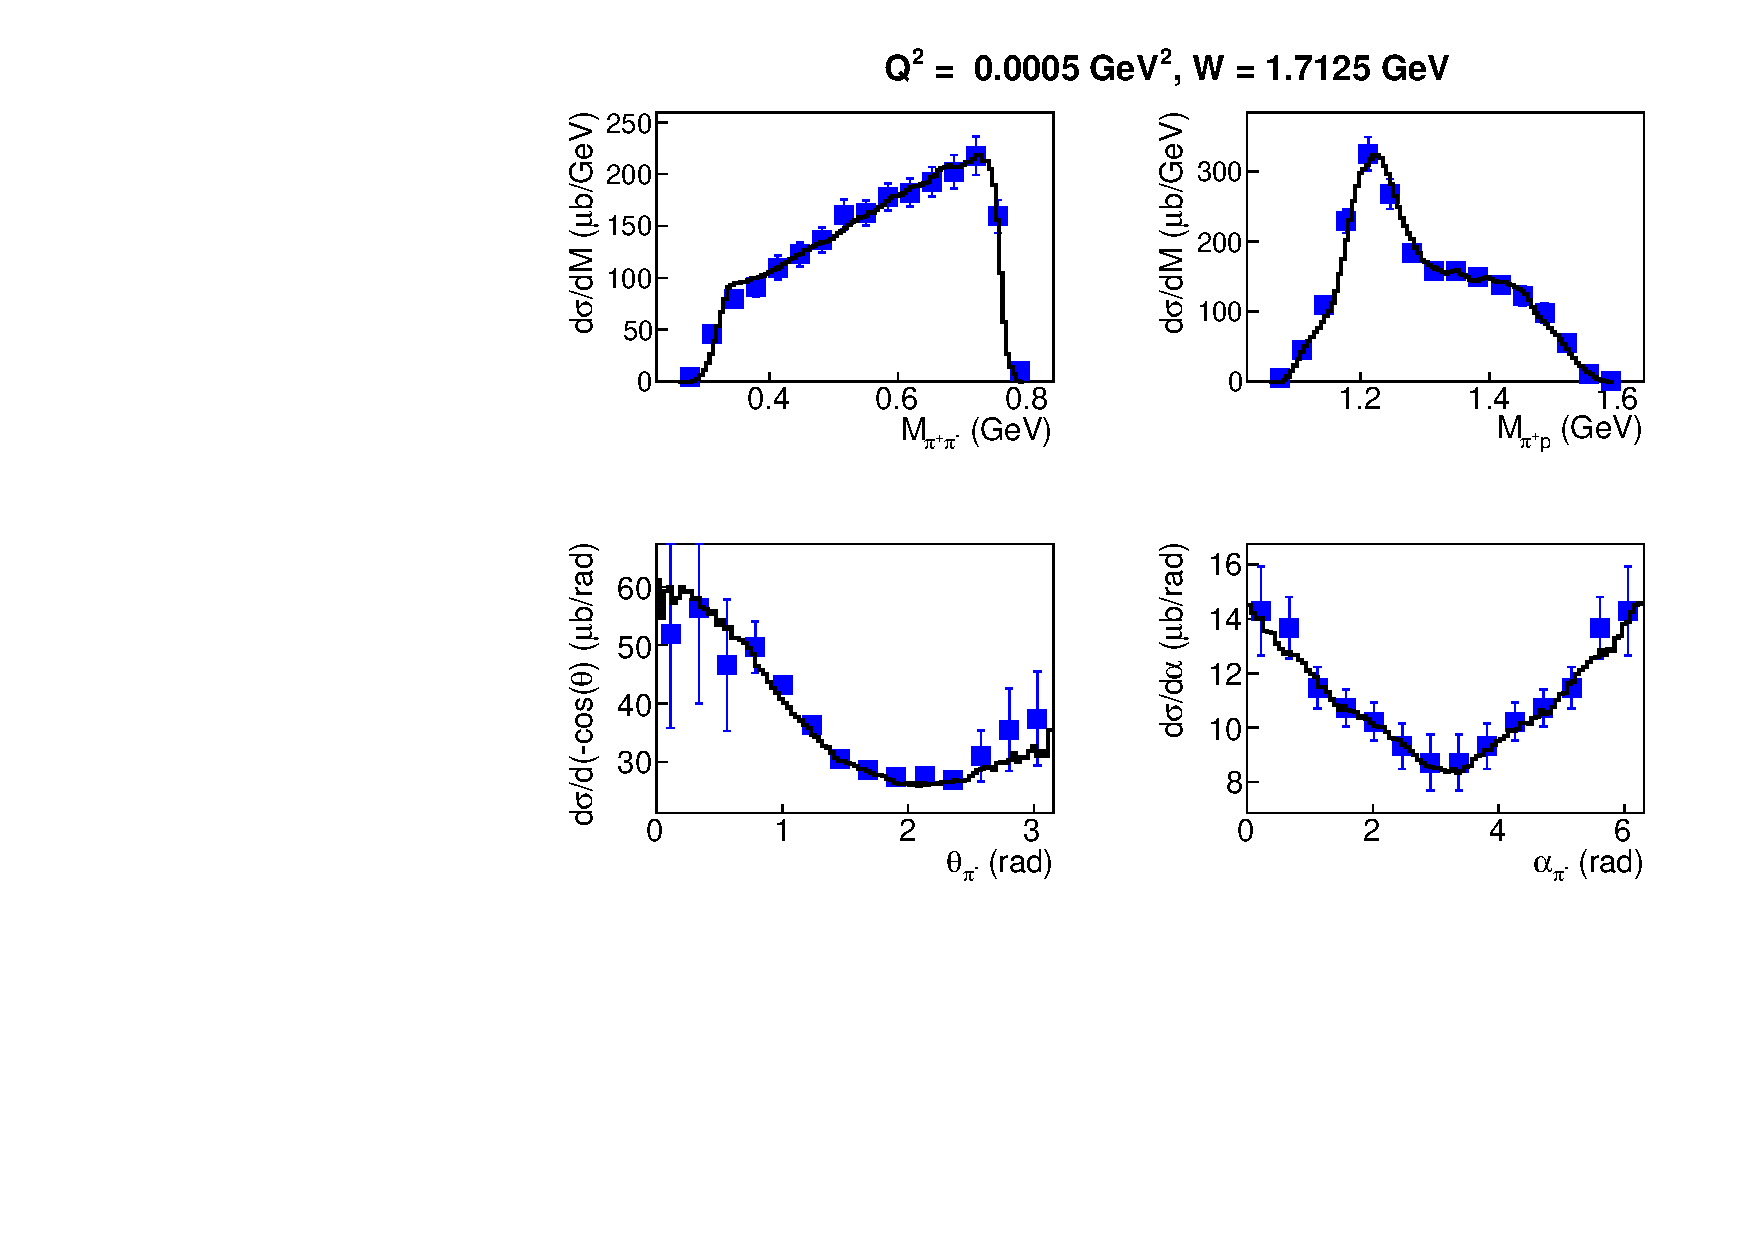
\includegraphics[height=0.45\textwidth]{pictures/quality/gol_17125.pdf}

}
\end{center}
\vspace{-0.6cm}
\caption{\small Comparison of the TWOPEG event distributions (curves) for the $W$ bin [1.7,~1.725]~GeV and $Q^2$ bin [0.0004,~0.0006]~GeV$^2$ with the single-fold differential experimental cross sections~\cite{Golovach:note} (squares) for the $W = 1.7125$~GeV, $Q^2 = 0$~GeV$^2$ point. This comparison corresponds to the data-set 2a, which is marked in Fig.~\ref{fig:gen_cover} by the green line.}
\label{fig:eg_gol_17125}
\end{figure}



\begin{figure}[!ht]
\begin{center}
\frame{
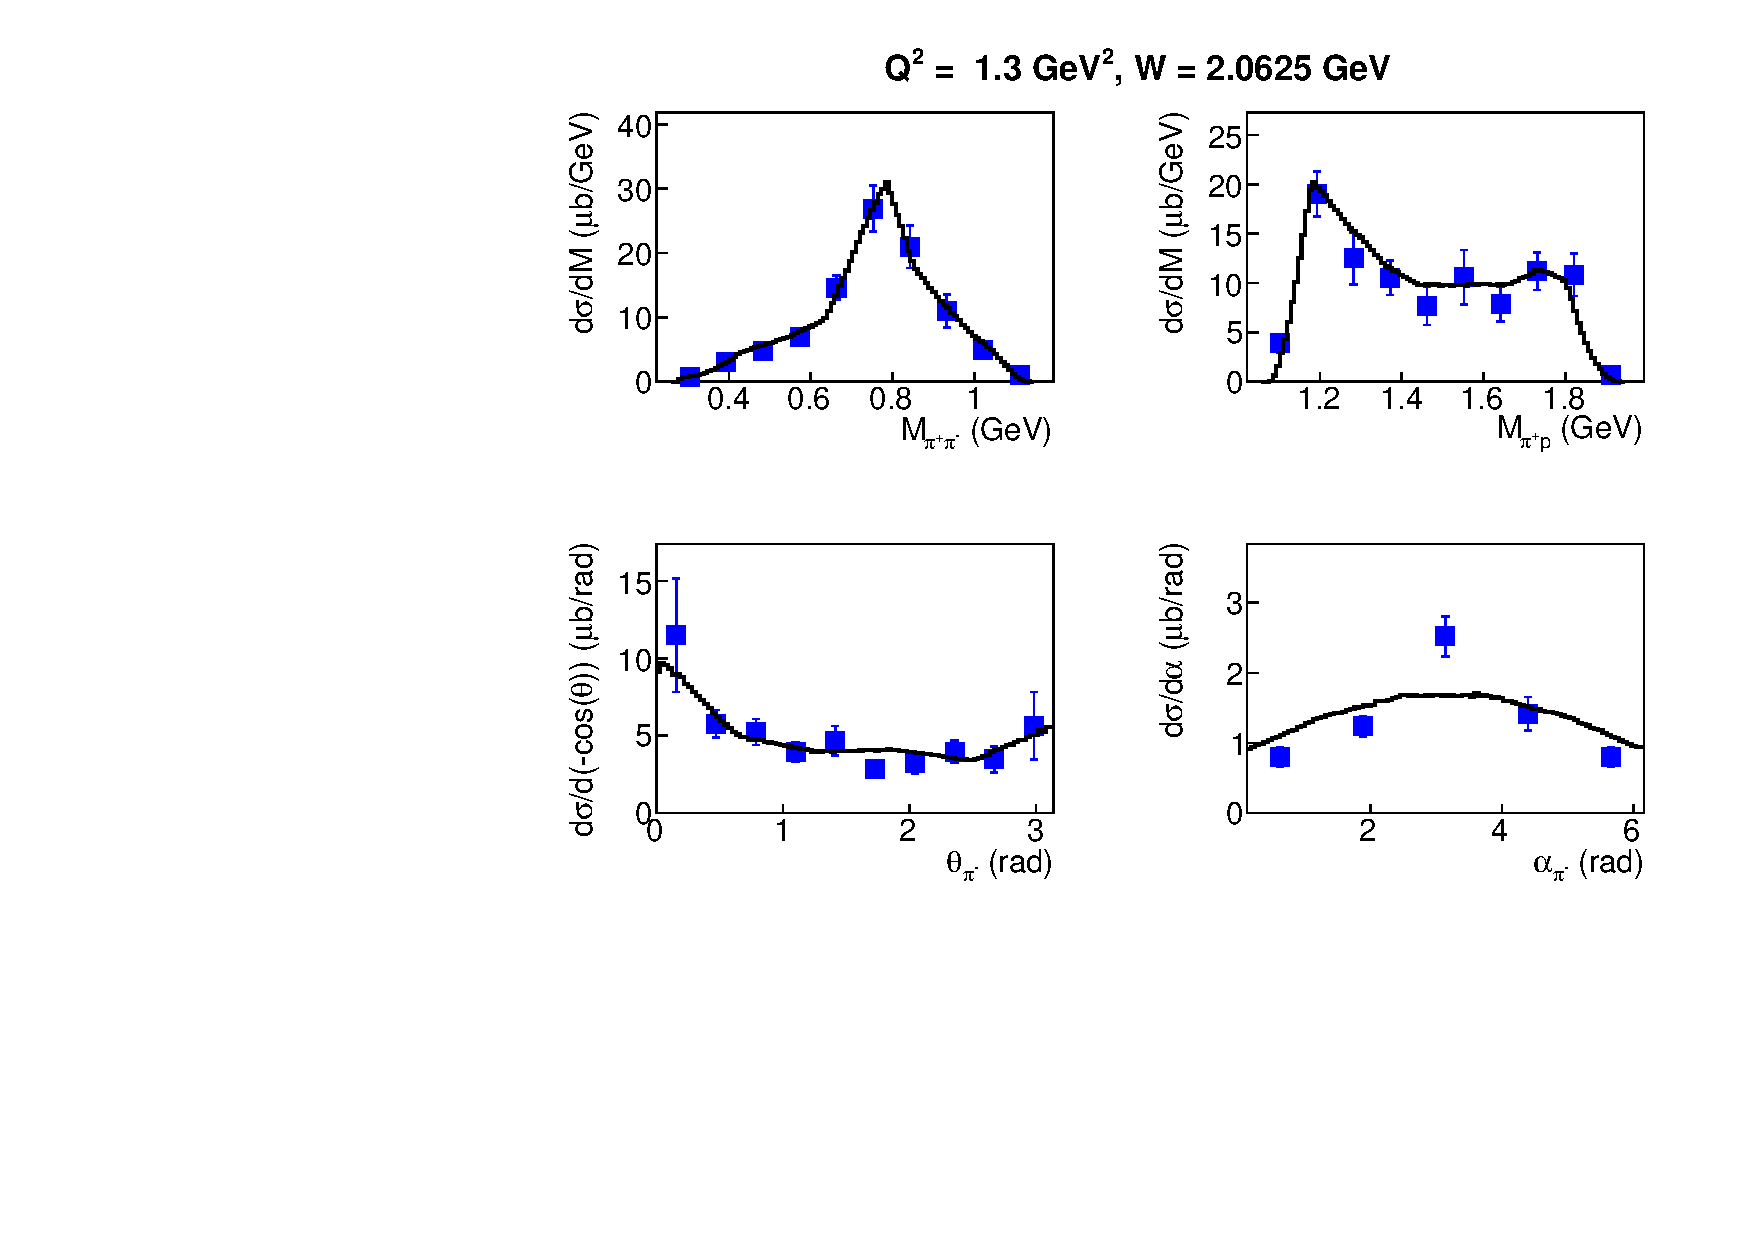
\includegraphics[height=0.45\textwidth]{pictures/quality/rip_130_20625.pdf}

}
\end{center}
\vspace{-0.6cm}
\caption{\small Comparison of the TWOPEG event distributions (curves) for the $W$ bin [2.05,~2.075]~GeV and $Q^2$ bin [1.25,~1.35]~GeV$^2$ with the single-fold differential experimental cross sections~\cite{Ripani:2002ss} (squares) for the $W = 2.0625$~GeV, $Q^2 = 1.3$~GeV$^2$ point. The TWOPEG distributions were obtained for $E_{beam} = 4$ GeV. This comparison corresponds to the red line at $Q^2 = 1.3$~GeV$^2$, that is adjacent to the data-set 1a in Fig.~\ref{fig:gen_cover}.}
\label{fig:eg_rip_130_20625}
\end{figure}

\begin{figure}[!ht]
\begin{center}
\frame{
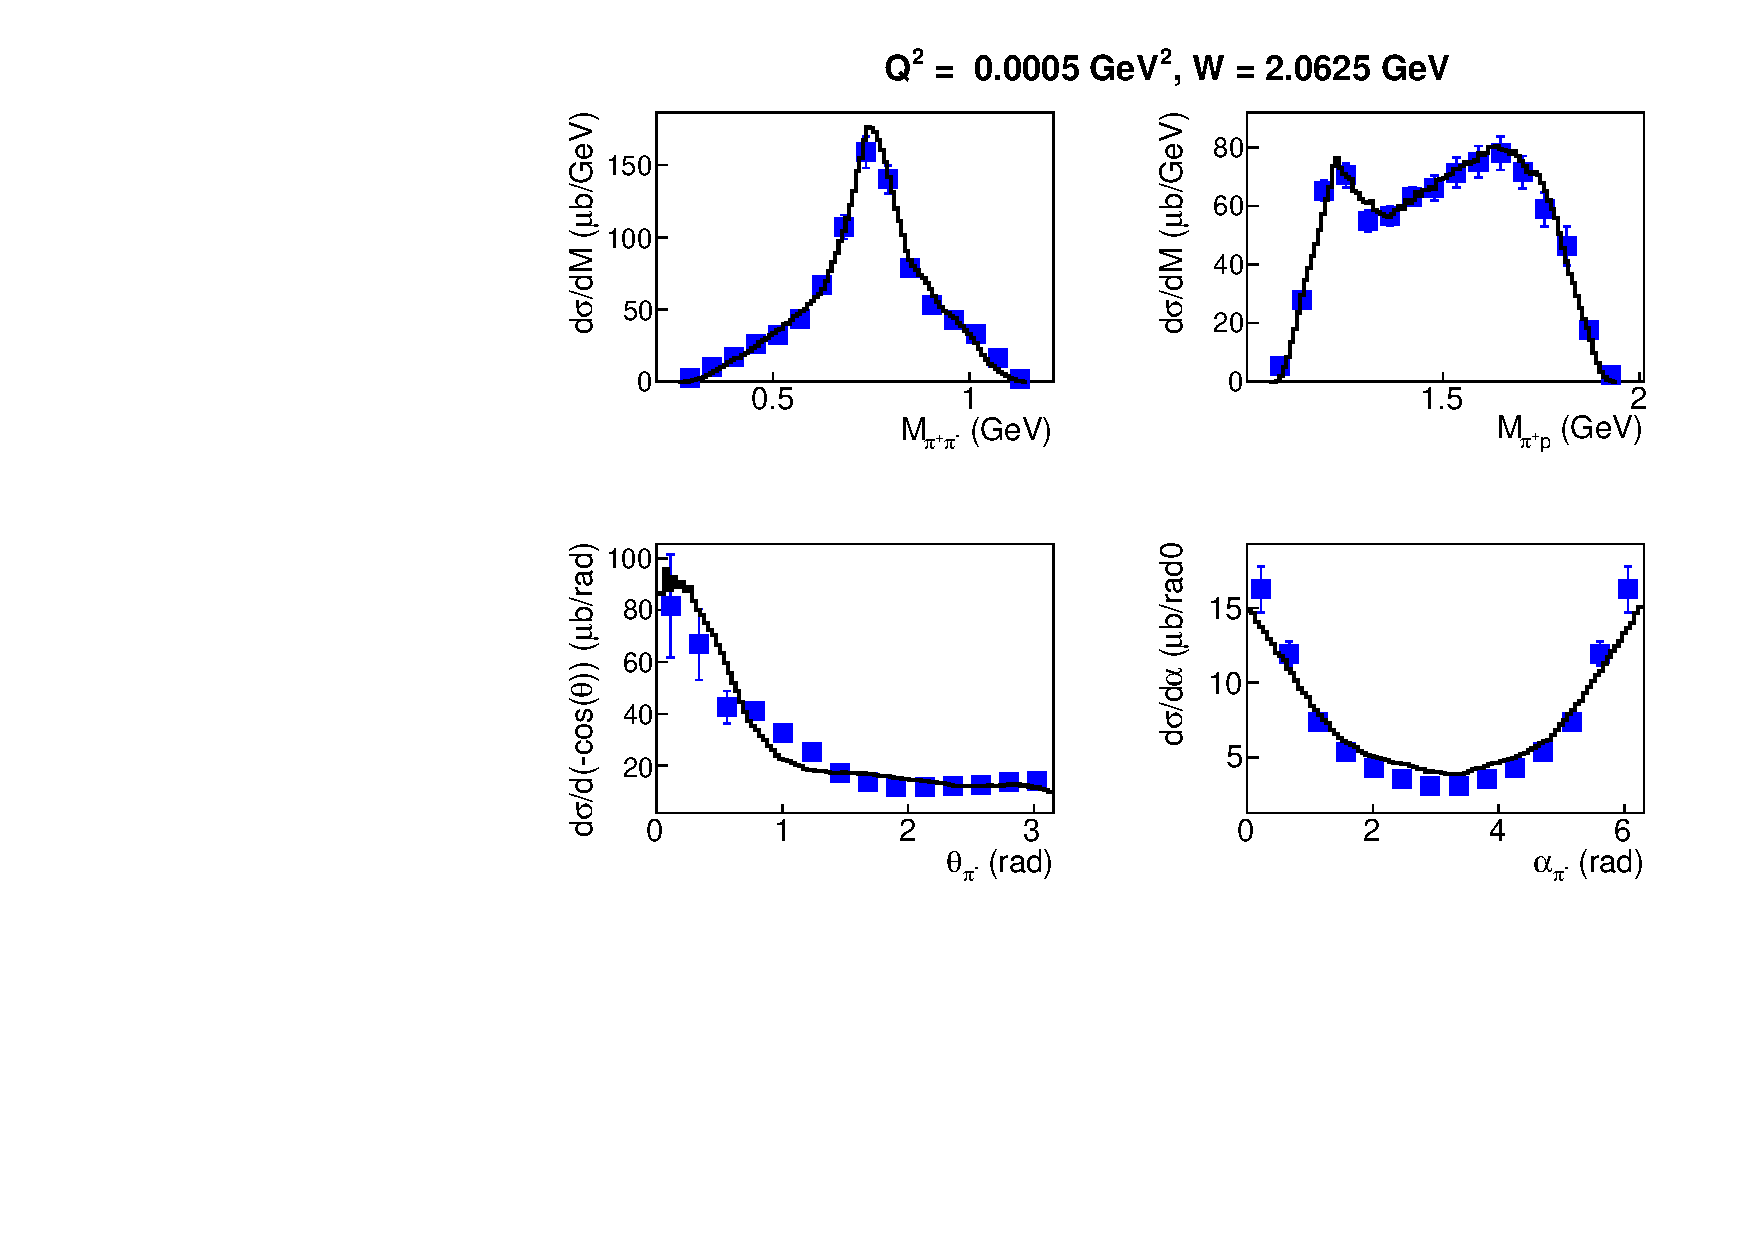
\includegraphics[height=0.45\textwidth]{pictures/quality/gol_20625.pdf}

}
\end{center}
\vspace{-0.6cm}
\caption{\small Comparison of the TWOPEG event distributions (curves) for the $W$ bin [2.05,~2.075]~GeV and $Q^2$ bin [0.0004,~0.0005]~GeV$^2$ with the single-fold differential experimental cross sections~\cite{Golovach:note} (squares) for the $W = 2.0625$~GeV, $Q^2 = 0$~GeV$^2$ point. This comparison corresponds to the data-set 2a, which is marked in Fig.~\ref{fig:gen_cover} by the green line.}
\label{fig:eg_gol_20625}
\end{figure}


\begin{figure}[!ht]
\begin{center}
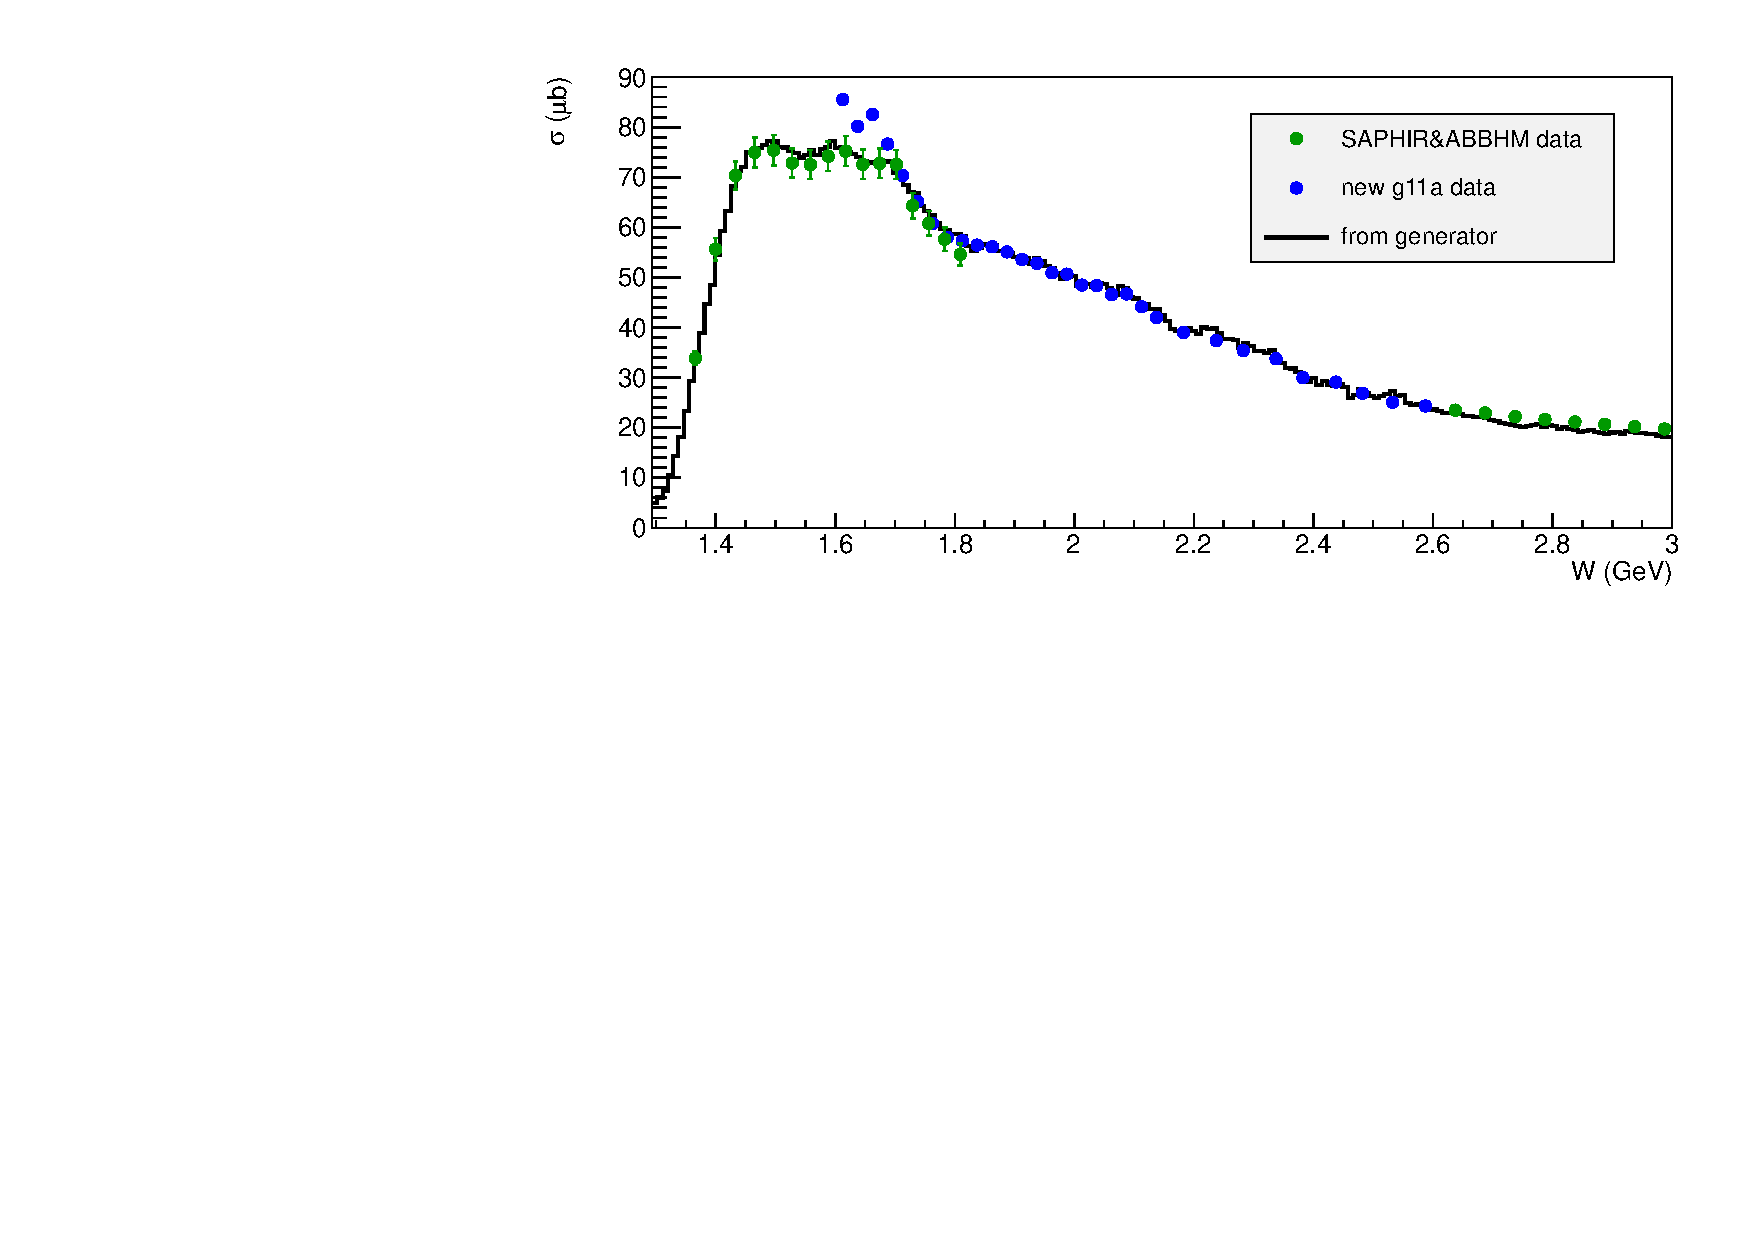
\includegraphics[width=0.65\textwidth]{pictures/quality/photon_point_gen_comp.pdf}
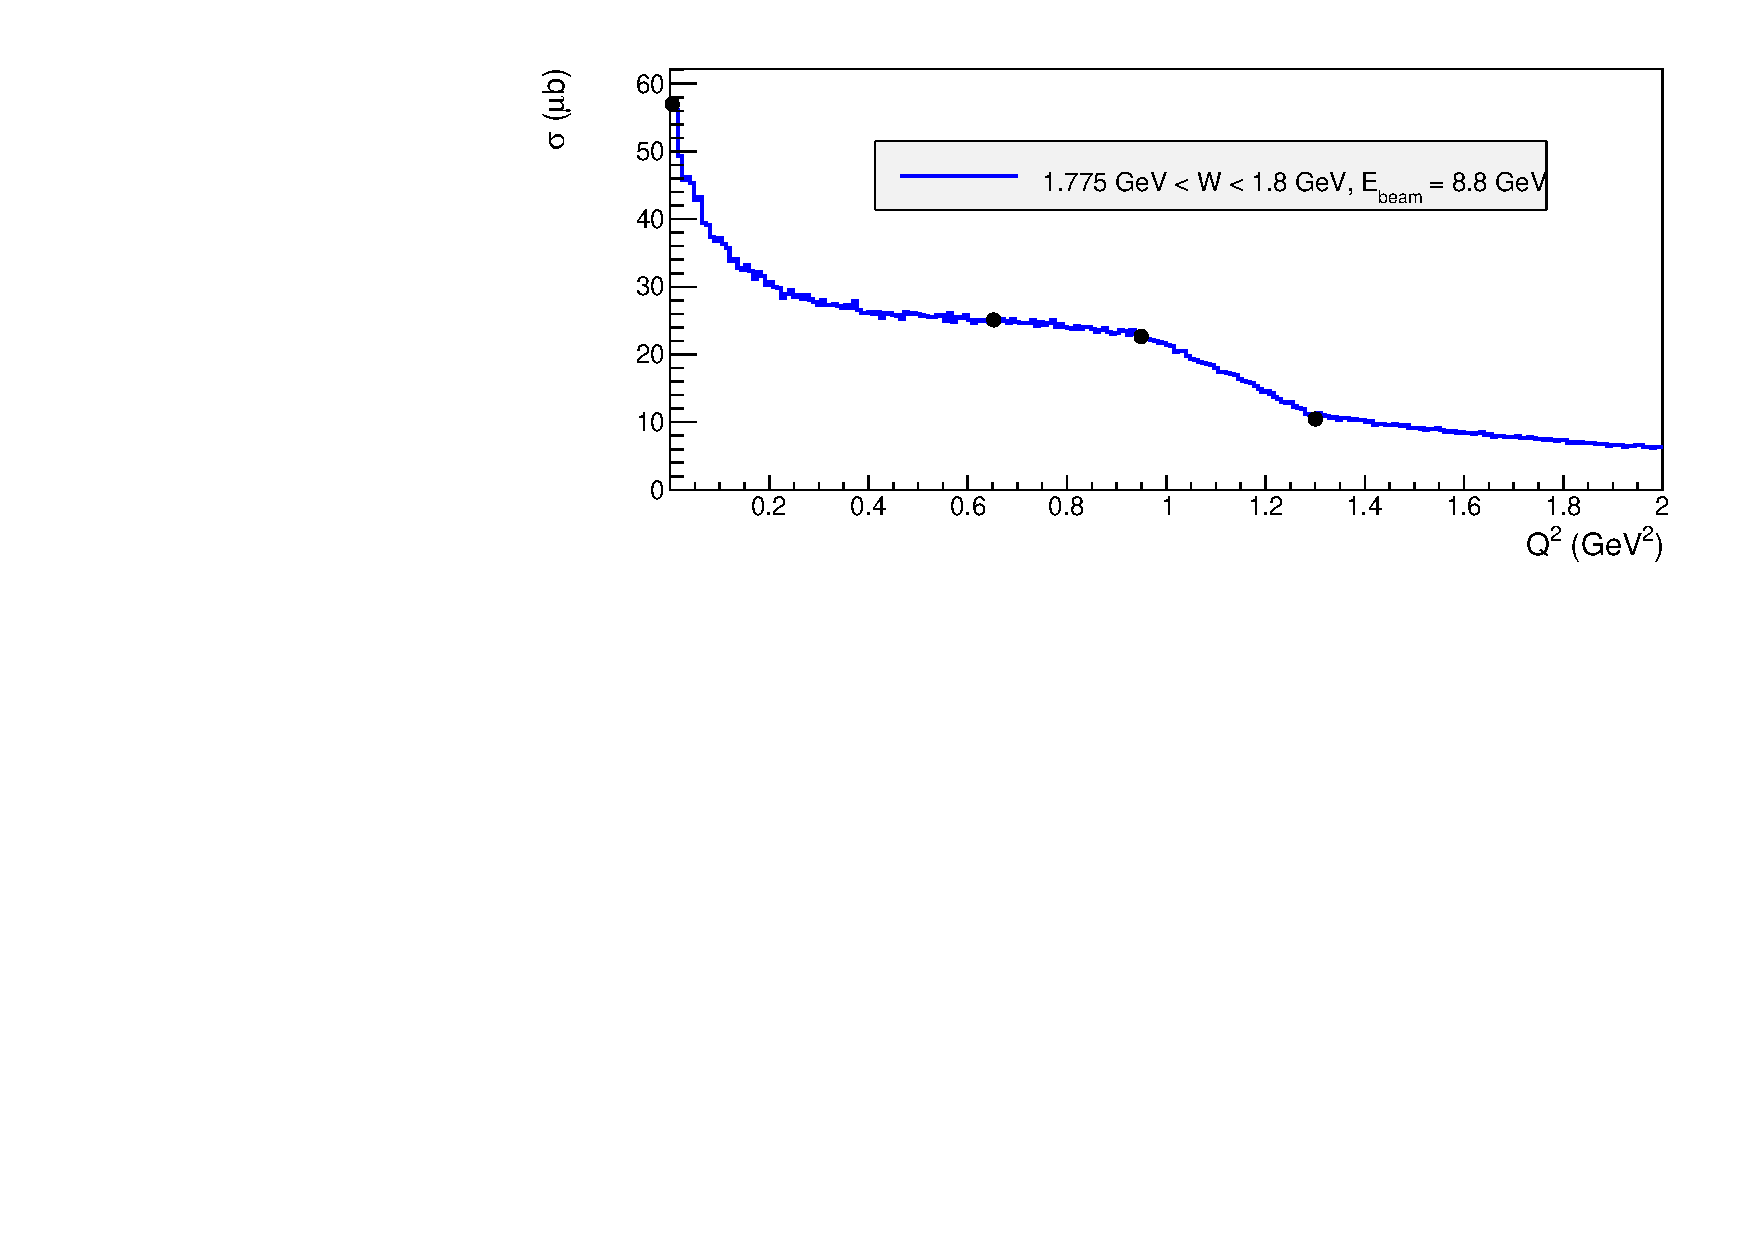
\includegraphics[width=0.65\textwidth]{pictures/quality/q2_dep_gen_comp.pdf}
\end{center}
\vspace{-0.6cm}
\caption{\small Upper plot shows the $W$ dependence of the integrated cross section for quasi-real photons with $Q^2$ [0.0004,~0.0005]~GeV$^2$ in comparison with data~\cite{Golovach:note,Wu:2005wf,ABBHHM:1968aa}. Lower plot shows a typical example of $Q^2$ dependence of the total cross section for one $W$ bin in comparison with the JM model~\cite{Mokeev:2015lda}  at $W = 1.7875$~GeV for a beam energy of 8.8~GeV.}
\label{fig:eg_ph_point}
\end{figure}




